\documentclass[frenchb]{beamer}
\usepackage{array}
\usepackage[utf8]{inputenc}
\usepackage{babel}
\usepackage[T1]{fontenc}
\usepackage{svg}

\usecolortheme{whale}
\title{TX-TIPE Chariot}
\subtitle{Etude et optimisation du parcours d'un chariot :\\conception d'un algorithme de cheminement}
\date{P19\\15 Juillet 2019}
\institute{Lycée Pierre d'Ailly - Université de Technologie de Compiègne}
\author{Romain Maliach-Auguste}
\begin{document}
\frame{\titlepage}
\begin{frame}
	\huge{Problématique:\\}
	\guillemotleft Optimiser la trajectoire d'un chariot élévateur\guillemotright
\end{frame}
  \begin{frame}
    \frametitle{Présentation du travail effectué}
	  \begin{itemize}
			 \item Implémentation des résultats mécaniques de mon binôme
			 \item Simplification du modèle de la grille et détermination d'une structure de données adaptée
			 \item Adaptation d'algorithmes connus et prouvés au problème
			 \item Implémentation et tests
	  \end{itemize}
  \end{frame}
  \begin{frame}
	  \frametitle{Résultats mécaniques de mon binôme}
	  \textbf{Durée minimale en virage}
	  	\[t_1 = \pi\sqrt{\frac{R_c(r+e)}{2lg}}\]
		où l est l'écart des roues, $R_c$ est le rayon de courbure, $r$ est le rayon des roues, $e$ la hauteur du colis (assimilé au centre de gravité).

	\textbf{Durée minimale en ligne droite}
		\[t_2=2\sqrt{\frac{d}{fg}}\]
		où $d$ est la longueur du couloir et $f$ le coefficient de frottement.
	 
	  \begin{figure}
		  \centering
		  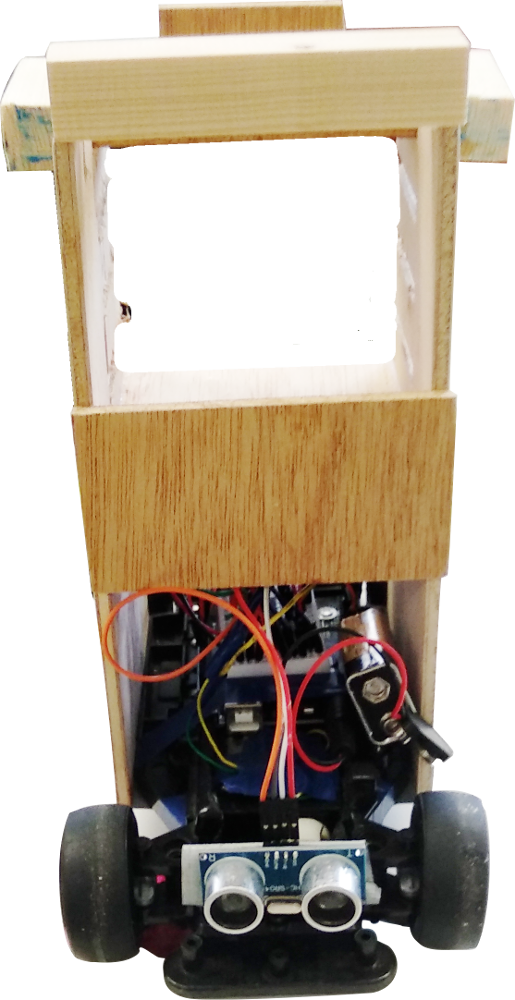
\includegraphics[height=2cm]{protoChariot.png}
		  \caption{Le modèle réduit utilisé pour nos tests}
	  \end{figure}
  \end{frame}
  \begin{frame}
	  \frametitle{Calcul numérique}
	  \begin{itemize}
		  \item numpy
		  \item networkx
	  \end{itemize}
  \end{frame}
  \begin{frame}
	  \frametitle{Modèle de la grille}
	  \begin{figure}
		  \centering
		  \includesvg[height=5cm]{grille1}
		  \caption{La grille et ses points d'arrêt}
		  \label{grille}
	  \end{figure}
  \end{frame}
  \begin{frame}
	  \frametitle{Simplification de la grille}
	  On sait qu'il faut minimiser les virages, donc on peut déjà sélectionner le meilleur chemin pour chaque couple de points:
	  \begin{figure}
		  \includesvg[height=5cm]{grille5}
		  \centering
	  \end{figure}
  \end{frame}
  \begin{frame}
	  \frametitle{Réduction de la grille en un graphe simplifié}
	  On peut alors perdre les chemins qui ne seront jamais utilisés, et pré-valuer en temps des chemins \textbf{localement} optimaux qui seront peut-être utilisés.
	  \begin{figure}
		  \centering
		  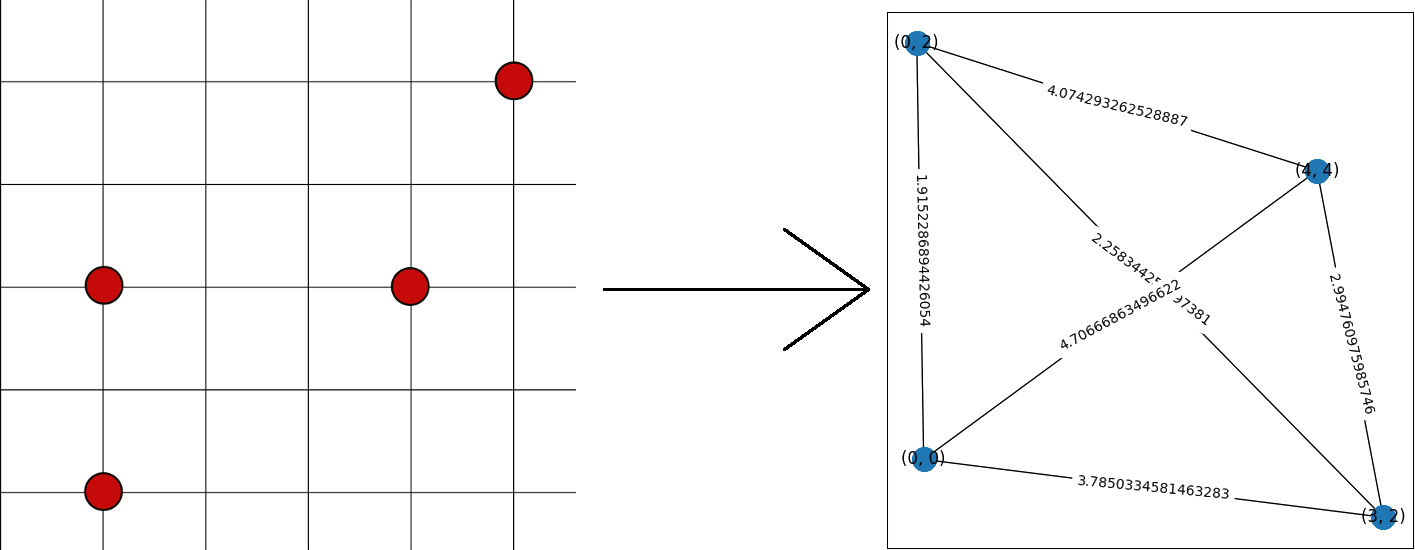
\includegraphics[width=11cm]{grapheSimp.png}
	  \end{figure}
	  On a un graphe fortement connexe, mais avec beaucoup moins de sommets.
  \end{frame}
  \begin{frame}
	  \frametitle{L'algorithme de Dijkstra}
	L'algorithme de Dijkstra calcule le meilleur chemin entre deux sommets d'un graphe non orienté.
	  \begin{figure}
		  \centering
		  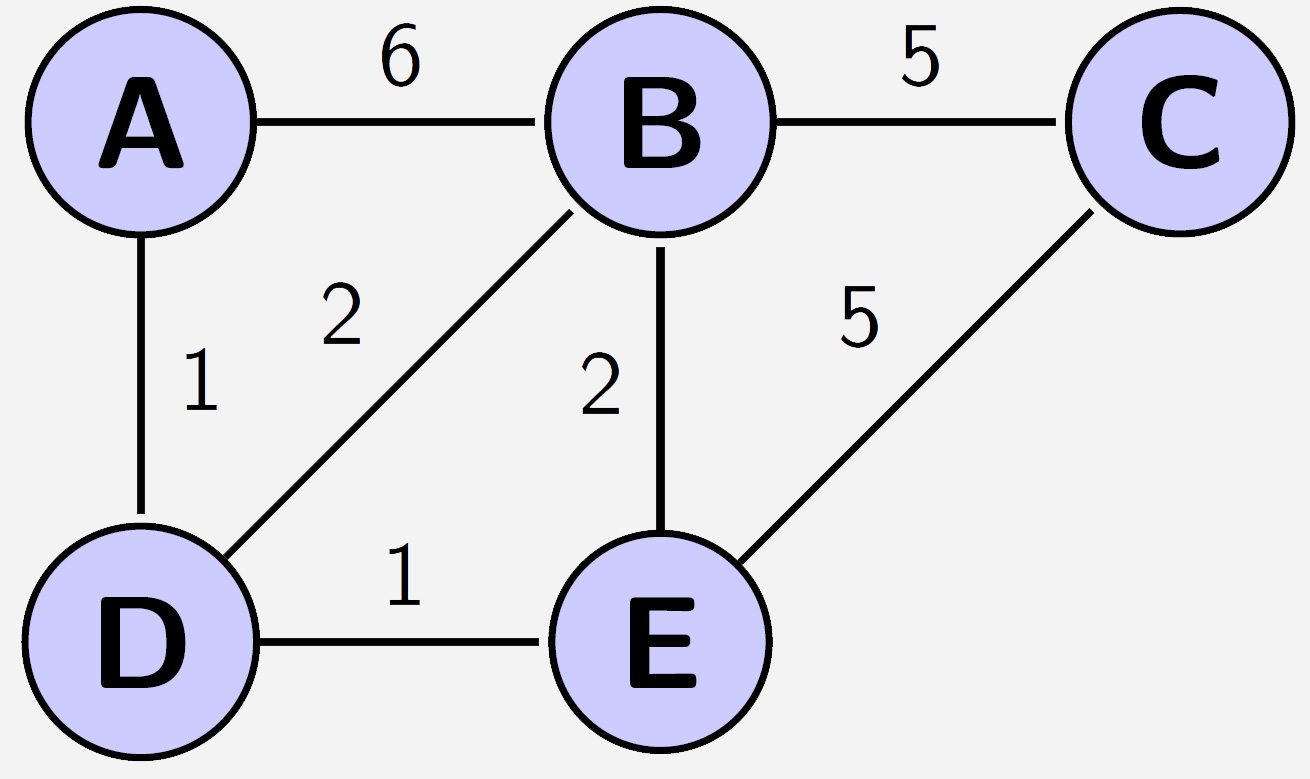
\includegraphics[height=4cm]{dijkstraExemple.png}
	  \end{figure}
  
  \end{frame}
  \begin{frame}
	  \frametitle{Adaptation de Dijkstra}
	  Mais il ne tient pas compte
	  \begin{itemize}
		  \item de l'optimisation locale réalisée à l'étape précédente
		  \item du coût supplémentaire d'un virage
	  \end{itemize}
	  On l'adapte donc ainsi: à chaque calcul de distance tentée, on additionne le coût du virage (le cas échéant), et on sait qu'à chaque itération l'arête de valuation minimale fera partie du chemin de valuation minimale.
  \end{frame}
  \begin{frame}
	  \frametitle{Démonstration}
	  {\huge main.py}
  \end{frame}

\end{document}
